\documentclass[aspectratio=169, 10pt]{beamer}

\usetheme{focus}

% Paleta SupaClock, consistente con Entrega 3 y Entrega 4
\definecolor{main}{RGB}{57, 110, 184}
\definecolor{background}{RGB}{255, 255, 255}
\definecolor{accent}{RGB}{63, 185, 80}
\definecolor{warn}{RGB}{218, 54, 51}
\definecolor{softgray}{RGB}{245, 247, 250}
\definecolor{darkink}{RGB}{23, 32, 51}
\definecolor{muted}{RGB}{91, 102, 122}

\setbeamercolor{alerted text}{fg=warn}

\usepackage[spanish]{babel}
\usepackage[utf8]{inputenc}
\usepackage[T1]{fontenc}
\usepackage{graphicx}
\usepackage{booktabs}
\usepackage{array}
\usepackage{tabularx}
\usepackage{tikz}
\usepackage{pgfplots}
\usepackage{pgf-pie}
\usepackage{pifont}
\pgfplotsset{compat=1.18}
\usetikzlibrary{shapes.geometric, arrows.meta, positioning, fit, backgrounds, calc, babel}

\setbeamerfont{itemize/enumerate body}{size=\small}
\setbeamerfont{itemize/enumerate subbody}{size=\footnotesize}
\setbeamerfont{block body}{size=\footnotesize}
\setbeamerfont{block title}{size=\small}

\graphicspath{{./}{../Entrega4/}{../Entrega3/}{../../mechanical/renders_v3/}{../../mechanical/}{../../hardware/SupaClock_Carrier_v4/}}

\newcommand{\metric}[2]{\textcolor{main}{\Large\textbf{#1}}\\[-0.02cm]{\scriptsize #2}}
\newcommand{\chip}[1]{\tikz[baseline=(n.base)]\node[rounded corners=3pt, fill=main!10, draw=main!35, inner xsep=4pt, inner ysep=2pt] (n) {\scriptsize #1};}
\newcommand{\demolabel}{\textcolor{accent}{\textbf{Demo}}}

\title{Wearable ``SupaClock''}
\subtitle{Producto \textbar{} Especificaciones técnicas y Desarrollo}
\date{\today}
\author{Grupo 10}
\institute{Ingeniería Eléctrica}
\titlegraphic{\hfill
\includegraphics[height=1.8cm]{supaclock_logo_rayo.pdf}}

\begin{document}

\maketitle

\begin{frame}{Índice}
    \tableofcontents
\end{frame}

% =============================================================================
\section{SupaClock como producto}

\begin{frame}{Contexto y motivación}
    \begin{columns}[T]
        \column{0.52\textwidth}
        \footnotesize
        \textbf{Problema que atacamos}
        \begin{itemize}\itemsep0.13cm
            \item Alta tasa de sedentarismo y sobrepeso en Chile.
            \item Los relojes comerciales agregan muchas funciones no esenciales.
            \item Falta una plataforma compacta para medir, registrar y validar datos propios.
        \end{itemize}
        \vspace{0.18cm}
        \begin{block}{Enfoque SupaClock}
            Wearable compacto, biométrico 5 en 1 y conectado a un ecosistema móvil.
        \end{block}
        \column{0.48\textwidth}
        \centering
        
\includegraphics[width=0.90\linewidth]{supaclock_logo_rayo.pdf}
        \vspace{0.18cm}
        \scriptsize \chip{cero distracciones}\quad \chip{datos propios}\quad \chip{uso diario}
    \end{columns}
\end{frame}

\begin{frame}{Funciones disponibles: de sensor a dato útil}
    \scriptsize
    \centering
    \renewcommand{\arraystretch}{1.25}
    \begin{tabular}{p{2.5cm}p{3.3cm}p{5.7cm}}
        \toprule
        \textbf{Función} & \textbf{Componente} & \textbf{Qué aporta} \\
        \midrule
        Temperatura & MAX30205 & Medición de contacto piel-sensor. \\
        BPM / SpO\textsubscript{2} & MAX30102 & Fotopletismografía roja/IR. \\
        Pasos & BMI160 & Movimiento inercial y algoritmo local. \\
        ML / HAR & ESP32-S3 + BMI160 & Clasificación de actividad física. \\
        ECG & AD8232 + ADC/DMA & Señal analógica acondicionada y enviada a la app. \\
        Interfaz & LCD táctil 1,28'' & Uso directo desde el reloj. \\
        \bottomrule
    \end{tabular}
    \vspace{0.35cm}
    \begin{block}{Idea clave}
        \scriptsize No es una lista de sensores: es una cadena completa de medición, procesamiento, visualización y registro.
    \end{block}
\end{frame}

\begin{frame}{Funciones del reloj}
    \footnotesize
    \begin{columns}[T]
        \column{0.50\textwidth}
        \textbf{Biométricas y actividad}
        \begin{itemize}\itemsep0.12cm
            \item Temperatura corporal.
            \item BPM y SpO\textsubscript{2}.
            \item Contador de pasos.
            \item ECG en reposo.
            \item Clasificación ML de actividad.
        \end{itemize}
        \column{0.50\textwidth}
        \textbf{Orquestación}
        \begin{itemize}\itemsep0.12cm
            \item ESP32-S3 coordina sensores y tareas.
            \item Pantalla LCD táctil capacitiva.
            \item BLE comunica reloj y app.
            \item Firmware modular por funciones.
        \end{itemize}
        \vspace{0.18cm}
        \begin{block}{\demolabel}
            Recorrer pantallas del reloj y mostrar mediciones disponibles.
        \end{block}
    \end{columns}
\end{frame}

\begin{frame}{Interacción con el reloj}
    \centering
    \begin{tikzpicture}[
        every node/.style={font=\tiny, align=center},
        display/.style={circle, draw=black!60, thick, fill=black!92, inner sep=0pt, minimum size=1.65cm},
        label/.style={below=0.02cm, font=\scriptsize},
        arr/.style={-{Latex[length=1.6mm]}, thick, main},
        garr/.style={-{Latex[length=1.6mm]}, thick, accent!70!black, dashed}
    ]
        % Fila principal: Watchface + 4 tiles
        \node[display] (wf) at (-5.6, 1.2) {\textcolor{white}{\scriptsize 12:37}\\[-0.05cm]\textcolor{main!45}{\tiny HR\,}\textcolor{warn!70}{\tiny 76}\\[-0.05cm]\textcolor{accent!70}{\tiny 4200}};
        \node[display] (hr) at (-2.8, 1.2) {\textcolor{warn!85}{\tiny RITMO}\\[-0.03cm]\textcolor{white}{\small 76}\\[-0.07cm]\textcolor{black!45}{\tiny bpm}};
        \node[display] (sp) at ( 0.0, 1.2) {\textcolor{main!60}{\tiny SpO\textsubscript{2}}\\[-0.03cm]\textcolor{white}{\small 97}\\[-0.07cm]\textcolor{black!45}{\tiny \%}};
        \node[display] (st) at ( 2.8, 1.2) {\textcolor{accent!85}{\tiny PASOS}\\[-0.03cm]\textcolor{white}{\small 4200}\\[-0.07cm]\textcolor{black!45}{\tiny /\,8k}};
        \node[display] (ac) at ( 5.6, 1.2) {\textcolor{main!60}{\tiny ACT.}\\[-0.03cm]\textcolor{white}{\tiny Caminar}\\[-0.07cm]\textcolor{black!45}{\tiny HAR}};
        \node[label] at (wf.south) {Watchface};
        \node[label] at (hr.south) {HR};
        \node[label] at (sp.south) {SpO\textsubscript{2}};
        \node[label] at (st.south) {Pasos};
        \node[label] at (ac.south) {Actividad};

        \draw[arr] (wf) -- (hr);
        \draw[arr] (hr) -- (sp);
        \draw[arr] (sp) -- (st);
        \draw[arr] (st) -- (ac);
        \node[font=\scriptsize] at (0, 2.6) {\emph{swipe L/R $\rightarrow$ carrusel de tiles}};

        % Fila inferior: Quick Panel + App Drawer + App
        \node[display] (qp)  at (-4.0, -2.0) {\textcolor{main!55}{\tiny brillo}\\[-0.05cm]\textcolor{white}{\tiny BLE ON}\\[-0.07cm]\textcolor{accent!70}{\tiny Tx IMU}};
        \node[display] (dw)  at ( 0.0, -2.0) {\textcolor{white}{\tiny ECG}\,\textcolor{warn!70}{\tiny\textbullet}\\[-0.05cm]\textcolor{white}{\tiny Batería}\\[-0.07cm]\textcolor{white}{\tiny Ajustes}};
        \node[display] (app) at ( 4.0, -2.0) {\textcolor{warn!80}{\tiny ECG}\\[-0.03cm]\textcolor{white}{\tiny \raisebox{-0pt}{\rule{0.45cm}{0.08cm}}}\\[-0.07cm]\textcolor{black!45}{\tiny live}};

        \node[label] at (qp.south)  {Quick Panel};
        \node[label] at (dw.south)  {App Drawer};
        \node[label] at (app.south) {App abierta};

        \draw[garr] (wf.south) to[bend right=20] node[left,font=\tiny]{swipe $\downarrow$} (qp.north);
        \draw[garr] (wf.south east) to[bend right=10] node[right,font=\tiny]{swipe $\uparrow$} (dw.north);
        \draw[garr] (dw) -- node[above,font=\tiny]{tap} (app);
        \draw[garr] (app.north east) to[bend left=25] node[right,font=\tiny]{botón atrás} (ac.south east);
    \end{tikzpicture}\\[0.10cm]
    \begin{minipage}{0.90\textwidth}
        \centering
        \scriptsize La \emph{watchface} es la raíz. Los 5 \emph{tiles} viven en un carrusel horizontal; \emph{swipe down} abre acceso rápido (brillo, BLE, Tx IMU) y \emph{swipe up} el cajón con 8 apps (ECG, actividad, temperatura, batería, ajustes, etc.).
    \end{minipage}
\end{frame}

\begin{frame}{Batería y autonomía}
    \scriptsize
    \begin{columns}[T]
        \column{0.32\textwidth}
        \textbf{Puntos técnicos}
        \begin{itemize}\itemsep0.06cm
            \item Batería LiPo de 300\,mAh.
            \item Carga y protección integradas en el XIAO ESP32-S3.
            \item MAX17048 fuel gauge estima carga y \emph{crate}.
            \item Detección automática de carga.
            \item Función de \emph{deep sleep} (apagado) con reactivación por botón.
            \item Carga completa en $\sim$4\,h por USB-C.
        \end{itemize}
        \column{0.34\textwidth}
        \centering
        \textbf{Descarga}\\[0.05cm]
        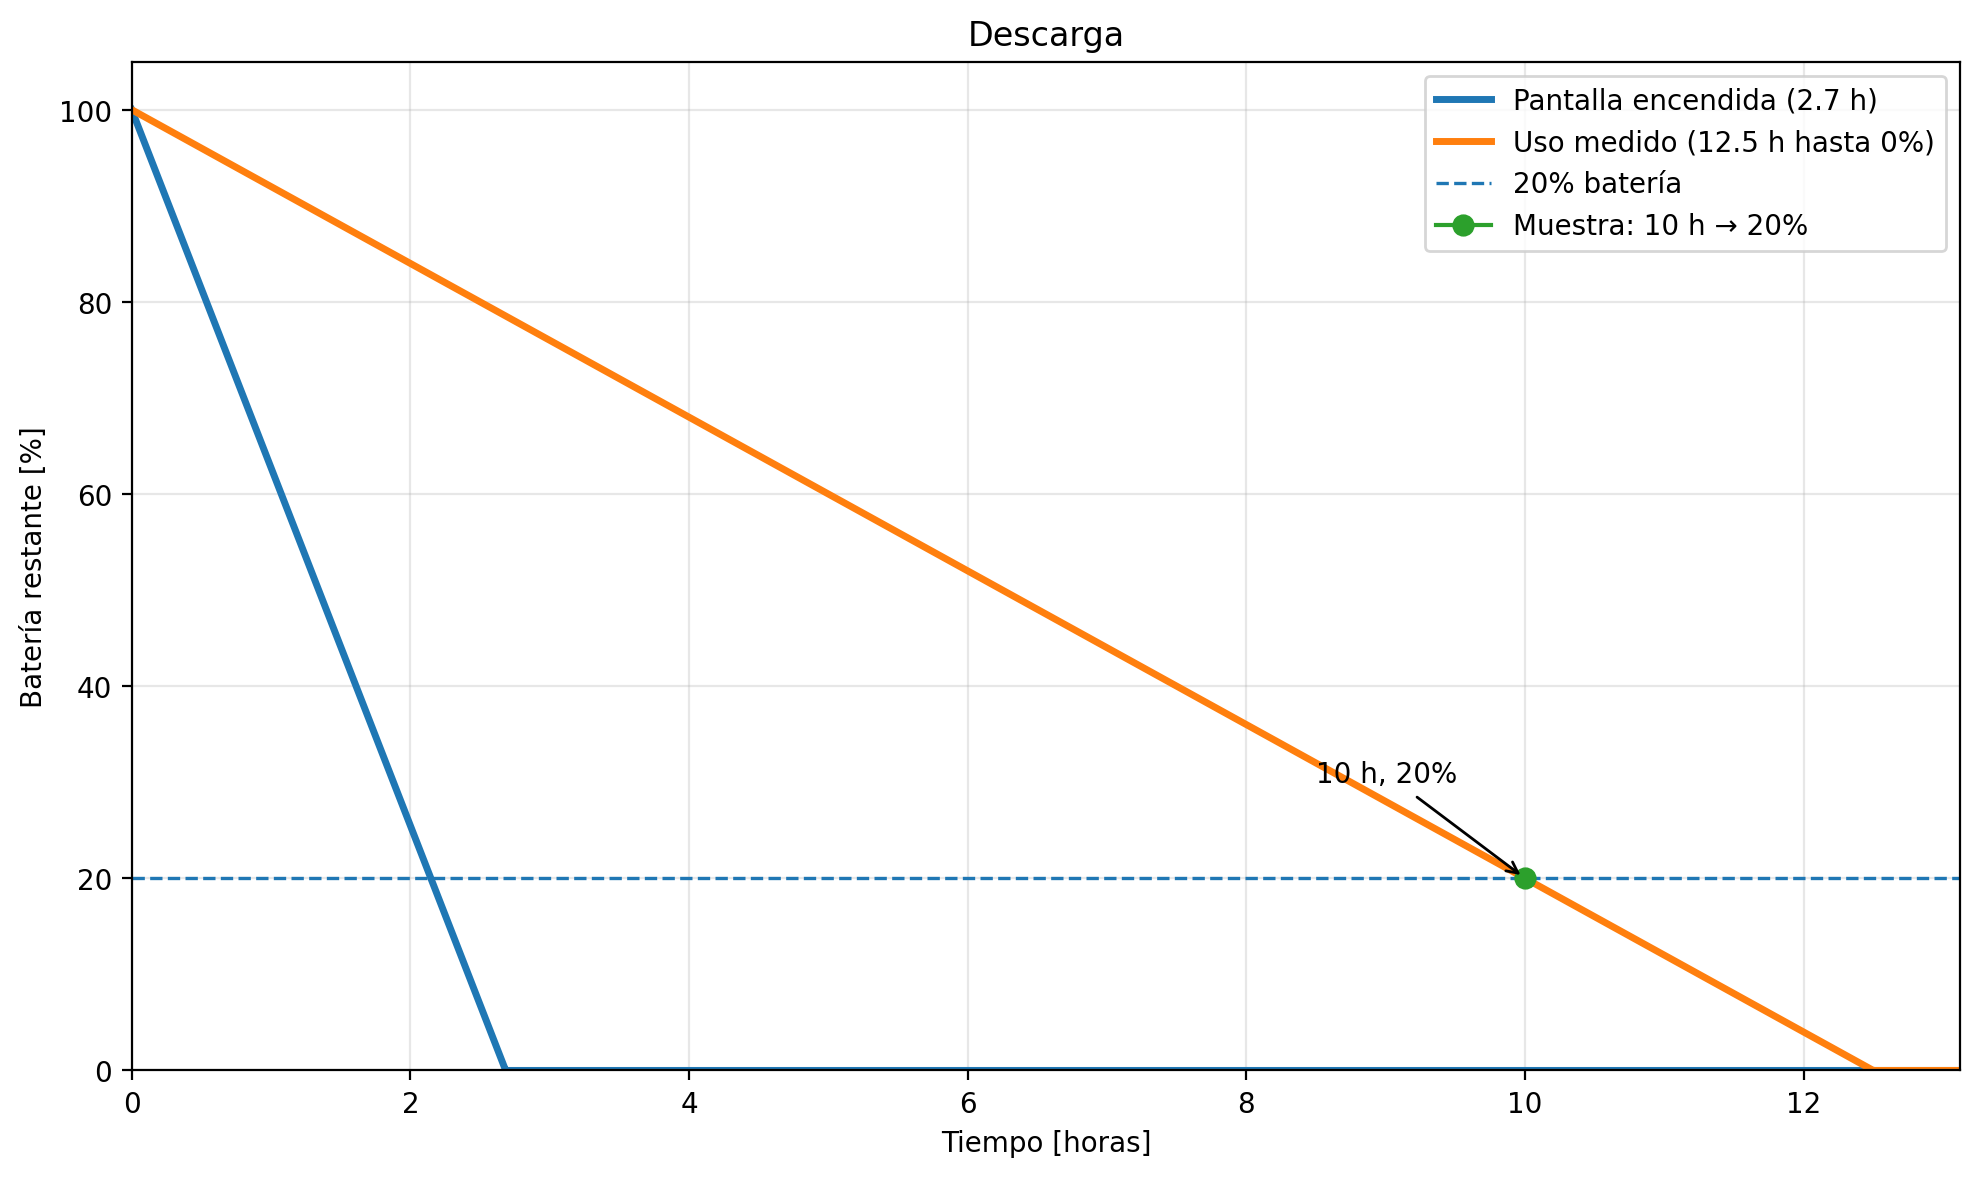
\includegraphics[width=\linewidth]{grafico_descarga_ajustado_10h_20pct.png}
        \column{0.34\textwidth}
        \centering
        \textbf{Carga}\\[0.05cm]
        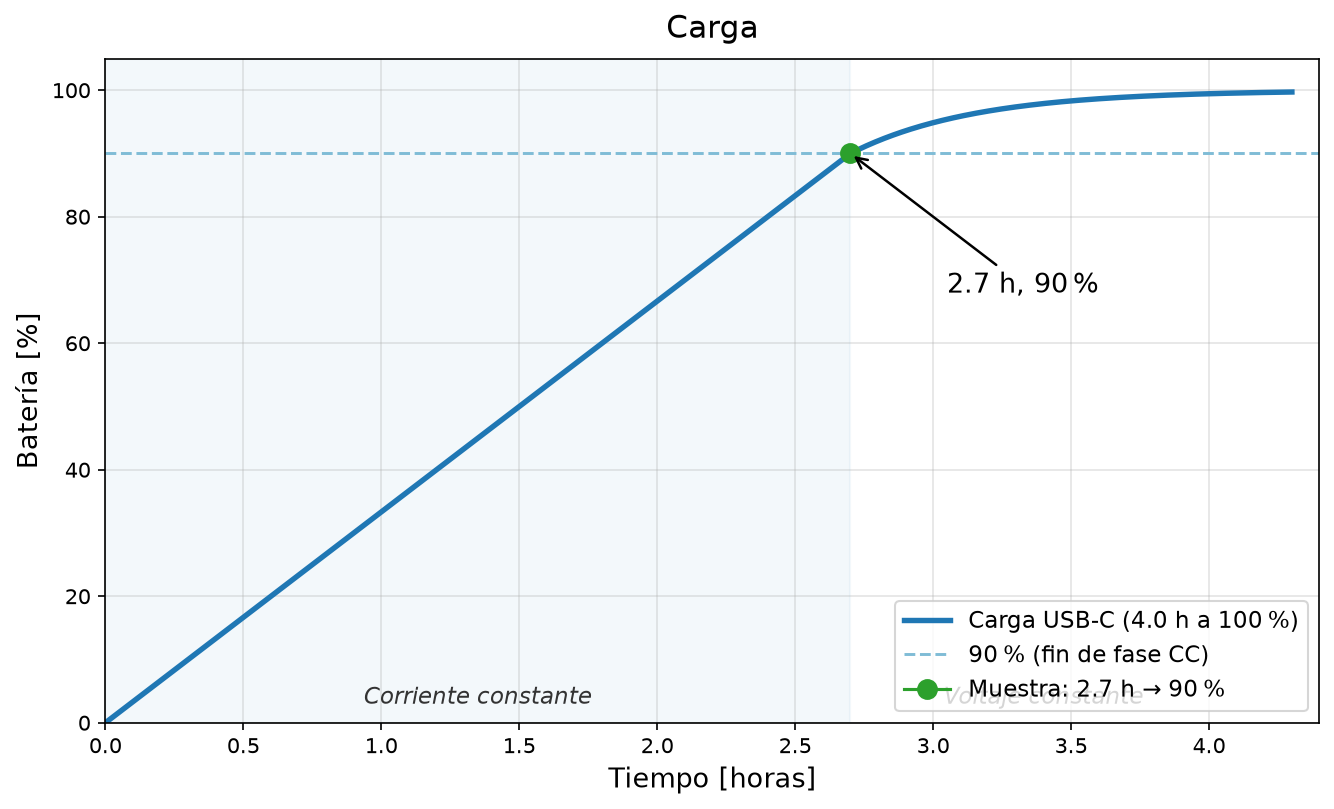
\includegraphics[width=\linewidth]{grafico_carga_ajustado.png}
    \end{columns}
    \vspace{0.10cm}
    \begin{center}
        \scriptsize
        \chip{\textbf{12,5\,h} uso mixto}\quad
        \chip{\textbf{2,7\,h} pantalla ON}\quad
        \chip{\textbf{4\,h} carga USB-C}\quad
        \chip{\textbf{$\sim$15\,\textmu A} deep sleep}
    \end{center}
\end{frame}

\begin{frame}{Consumo por subsistema}
    \scriptsize
    \centering
    \renewcommand{\arraystretch}{1.10}
    \begin{tabular}{p{3.6cm}p{2.5cm}r p{4.4cm}}
        \toprule
        \textbf{Subsistema} & \textbf{Modo} & \textbf{mA típ.} & \textbf{Fuente / control} \\
        \midrule
        XIAO ESP32-S3 activo & idle FreeRTOS & $\sim$30    & Datasheet Espressif ESP32-S3 \\
        XIAO ESP32-S3 deep sleep & RTC + ext1 wake & 0,014 & Con RTC\_PERIPH ON \\
        LCD GC9A01 + backlight & Brillo alto & 15--20      & GPIO PWM en firmware \\
        MAX30102 activo & PPG rojo/IR & 1,1                & Registro \texttt{MODE\_CONFIG} \\
        MAX30102 shutdown & Deep sleep & 0,001            & \texttt{MODE\_CONFIG} bit 7 \\
        BMI160 low-power & Acc + gyro & 0,13              & FIFO 50\,Hz \\
        BMI160 suspend & Deep sleep & 0,003               & \texttt{CMD\_ACC/GYR\_SUSPEND} \\
        MAX30205 activo & Conv continua & 0,6             & Registro CONFIG \\
        MAX30205 shutdown & Deep sleep & 0,001            & CONFIG bit 0 \\
        AD8232 & ECG activo & 0,17                         & Alimentado solo durante ECG \\
        BLE NimBLE advertising & \emph{connectable} & 5   & Conn interval 100\,ms \\
        \bottomrule
    \end{tabular}
    \vspace{0.15cm}
    \begin{block}{Cómo se llega a 12,5\,h}
        \scriptsize En modo típico (pantalla mayormente apagada, BLE conectado, HAR + IMU + PPG activos $\rightarrow$ $\sim$24\,mA promedio), 300\,mAh dan $\sim$12,5\,h. Con pantalla siempre encendida caen a 2,7\,h. Valores de datasheets; medición fina queda propuesta como trabajo futuro.
    \end{block}
\end{frame}

\begin{frame}{Carcasa, PCB y reducción de tamaño}
    \begin{columns}[T]
        \column{0.50\textwidth}
        \footnotesize
        \begin{itemize}\itemsep0.12cm
            \item Carcasa impresa en 3D con PLA.
            \item PCB fabricada en China para mejorar integración.
            \item Reducción de 28\,\% en el eje principal.
            \item Reducción de 36\,\% en volumen frente al prototipo inicial.
        \end{itemize}
        \vspace{0.15cm}
        \begin{block}{Dimensiones finales}
            \footnotesize \textbf{1,7\,cm $\times$ 7,4\,cm $\times$ 9,3\,cm} \\
            \scriptsize (alto $\times$ ancho $\times$ largo)
        \end{block}
        \column{0.50\textwidth}
        \centering
        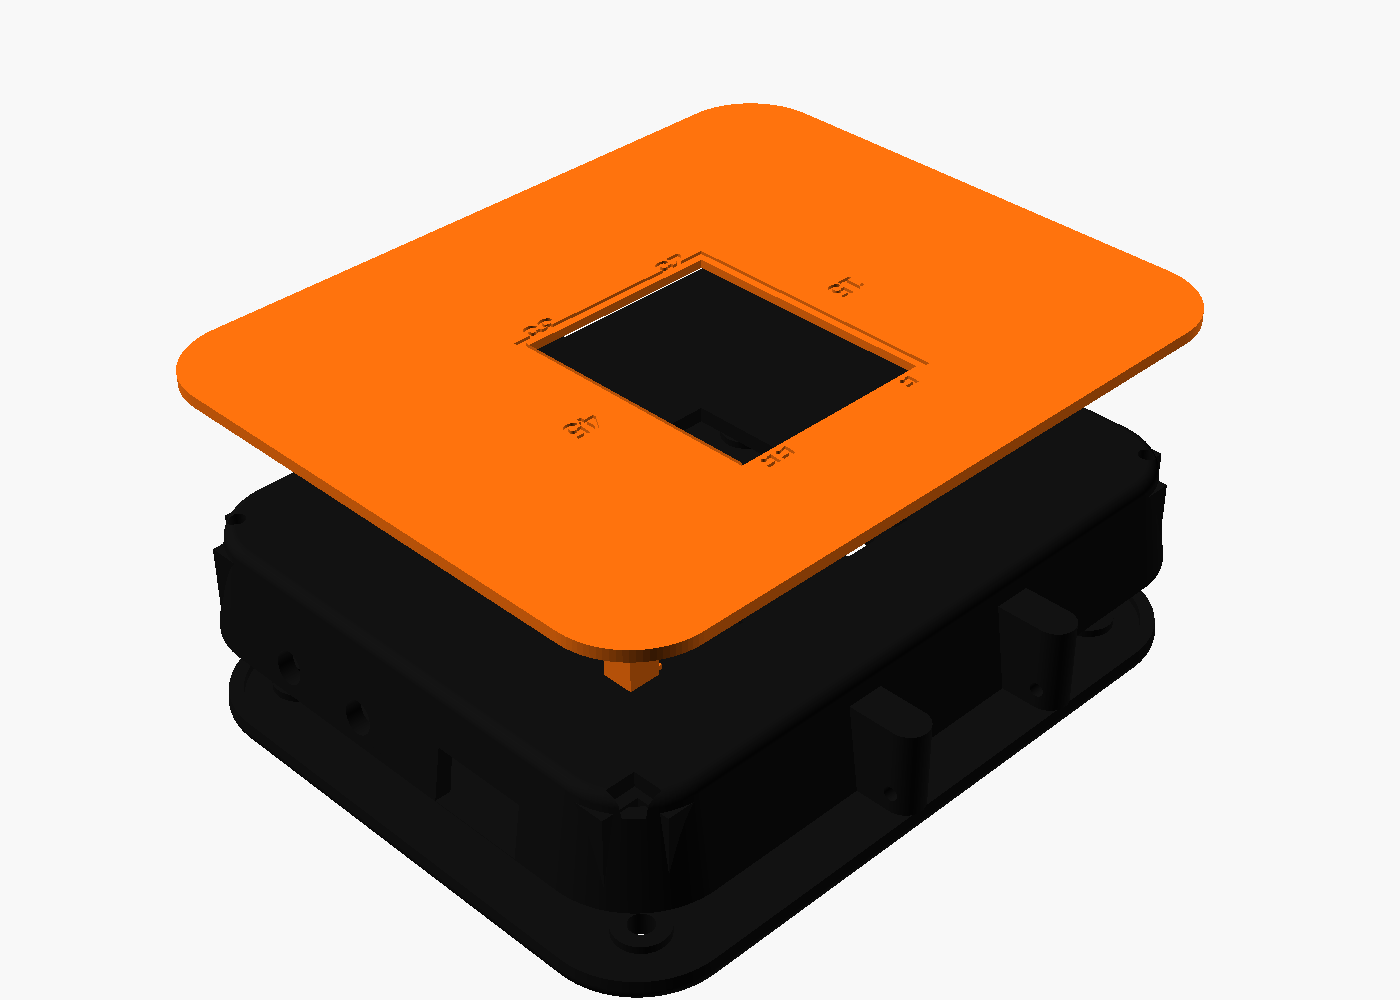
\includegraphics[width=0.90\linewidth]{v3_sport_snap_exploded_3layers.png}
        \vspace{0.2cm}
        \scriptsize PCB + sensores + batería + carcasa en una unidad cerrable.
    \end{columns}
\end{frame}

\begin{frame}{Aplicación móvil: entrada al ecosistema}
    \begin{columns}[T]
        \column{0.48\textwidth}
        \footnotesize
        \textbf{Qué se muestra primero}
        \begin{itemize}\itemsep0.12cm
            \item Inicio de sesión y acceso a usuario.
            \item Dashboard con métricas principales.
            \item Navegación hacia mediciones y modo desarrollador.
        \end{itemize}
        \vspace{0.2cm}
        \begin{block}{\demolabel}
            Login, pantalla principal y navegación por la app.
        \end{block}
        \column{0.52\textwidth}
        \centering
        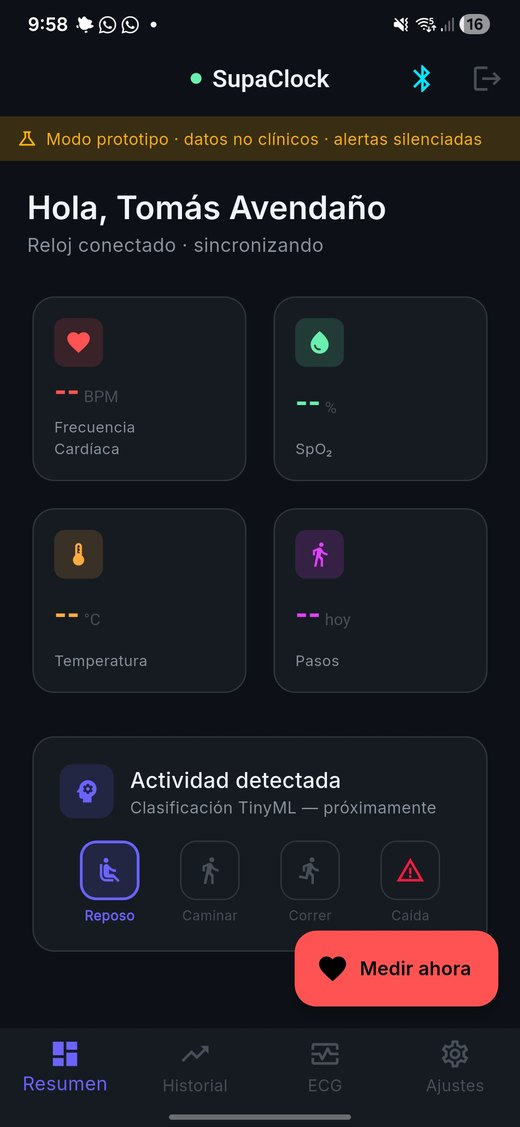
\includegraphics[width=0.31\linewidth]{app_home_e4.jpg}\hfill
        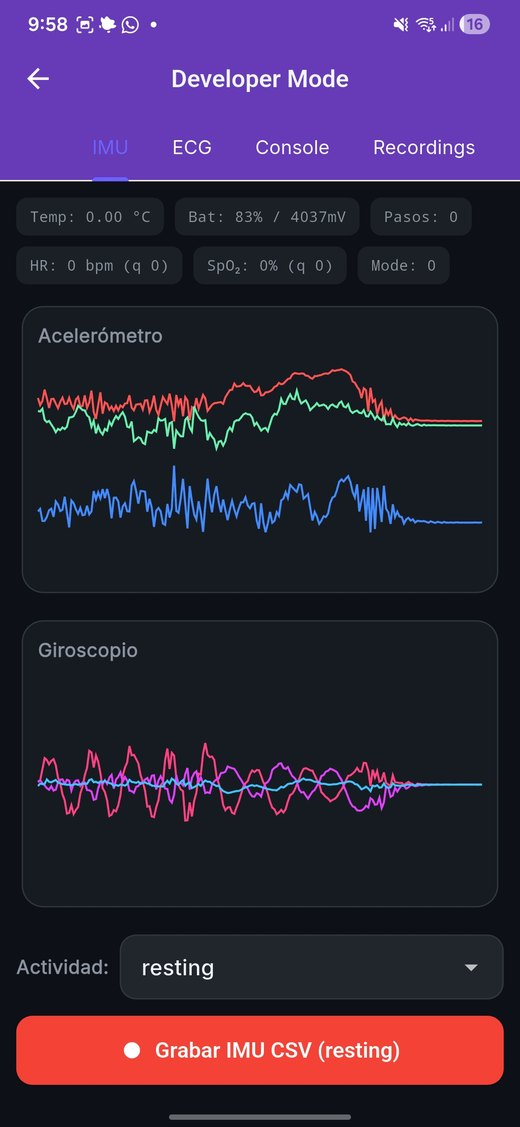
\includegraphics[width=0.31\linewidth]{app_imu_e4.jpg}\hfill
        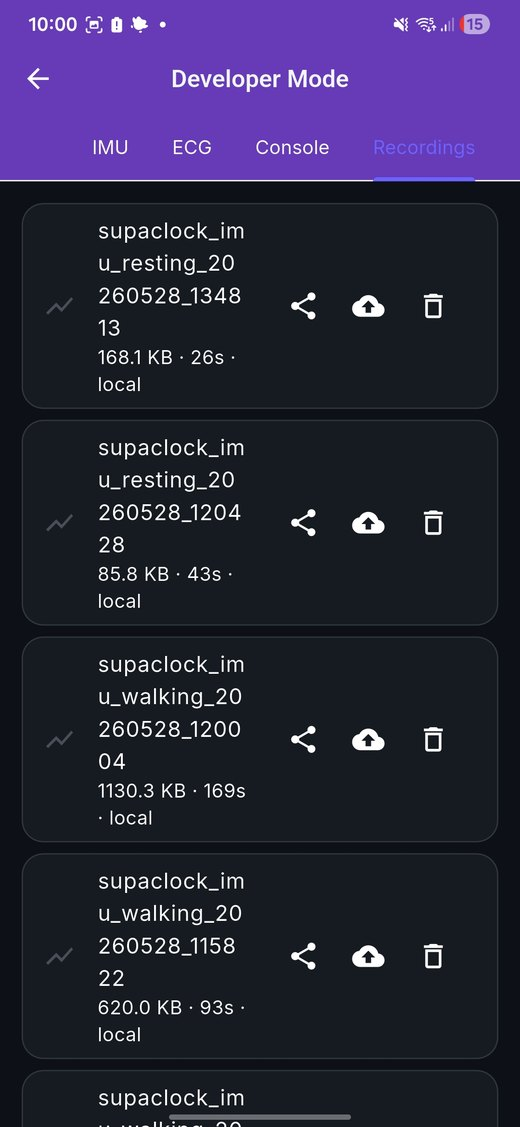
\includegraphics[width=0.31\linewidth]{app_rec_e4.jpg}
    \end{columns}
\end{frame}

\begin{frame}{Aplicación móvil: datos, BLE y registro}
    \begin{columns}[T]
        \column{0.55\textwidth}
        \footnotesize
        \begin{itemize}\itemsep0.13cm
            \item Conexión BLE con el reloj.
            \item Visualización de métricas y señales crudas.
            \item Grabación local de sesiones para validación.
            \item Puente hacia almacenamiento y análisis posterior.
        \end{itemize}
        \column{0.45\textwidth}
        \begin{tikzpicture}[node distance=0.35cm, every node/.style={font=\scriptsize}]
            \node[draw, rounded corners, fill=main!10, minimum width=3.7cm, minimum height=0.70cm] (watch) {SupaClock};
            \node[draw, rounded corners, fill=accent!10, below=of watch, minimum width=3.7cm, minimum height=0.70cm] (app) {Flutter App};
            \node[draw, rounded corners, fill=softgray, below=of app, minimum width=3.7cm, minimum height=0.70cm] (local) {CSV / historial local};
            \node[draw, rounded corners, fill=softgray, below=of local, minimum width=3.7cm, minimum height=0.70cm] (cloud) {Firebase / dataset};
            \draw[-{Latex[length=2mm]}, thick, main] (watch) -- node[right]{BLE} (app);
            \draw[-{Latex[length=2mm]}, thick, accent] (app) -- (local);
            \draw[-{Latex[length=2mm]}, thick, accent] (local) -- node[right]{sync} (cloud);
        \end{tikzpicture}
        \vspace{0.2cm}
        \begin{block}{\demolabel}
            Conectar, navegar, registrar y mostrar sesión.
        \end{block}
    \end{columns}
\end{frame}

% =============================================================================
\section{Machine Learning on-device}

\begin{frame}{HAR: arquitectura del modelo CNN 1D}
    \centering
    \resizebox{0.98\textwidth}{!}{%
    \begin{tikzpicture}[
        every node/.style={font=\tiny, align=center},
        inp/.style={rectangle, rounded corners=2pt, draw=black!60, thick, fill=softgray, minimum width=1.7cm, minimum height=1.0cm},
        conv/.style={rectangle, rounded corners=2pt, draw=black!70, thick, fill=main!25, minimum width=1.7cm, minimum height=1.0cm},
        pool/.style={rectangle, rounded corners=2pt, draw=black!70, thick, fill=main!10, minimum width=1.35cm, minimum height=1.0cm},
        gap/.style={rectangle, rounded corners=2pt, draw=black!70, thick, fill=warn!25, minimum width=1.35cm, minimum height=1.0cm},
        dense/.style={rectangle, rounded corners=2pt, draw=black!70, thick, fill=accent!25, minimum width=1.35cm, minimum height=1.0cm},
        soft/.style={rectangle, rounded corners=2pt, draw=black!70, thick, fill=accent!45, minimum width=1.6cm, minimum height=1.0cm},
        dims/.style={below=0.02cm, font=\tiny\itshape, text=black!55},
        arr/.style={-{Latex[length=1.8mm]}, thick, black!60}
    ]
        % Nodos horizontales
        \node[inp]   (in)  at (-6.9, 0) {\textbf{Entrada}\\ ventana\\ IMU};
        \node[conv]  (c1)  at (-5.0, 0) {\textbf{Conv1D}\\ 32 filtros\\ k=5, ReLU};
        \node[pool]  (p1)  at (-3.3, 0) {\textbf{MaxPool}\\ pool=2};
        \node[conv]  (c2)  at (-1.6, 0) {\textbf{Conv1D}\\ 64 filtros\\ k=5, ReLU};
        \node[pool]  (p2)  at ( 0.1, 0) {\textbf{MaxPool}\\ pool=2};
        \node[conv]  (c3)  at ( 1.8, 0) {\textbf{Conv1D}\\ 128 filtros\\ k=3, ReLU};
        \node[gap]   (gap) at ( 3.5, 0) {\textbf{GAP}\\ colapsa\\ tiempo};
        \node[dense] (d)   at ( 5.2, 0) {\textbf{Dense}\\ 64 + Dropout};
        \node[soft]  (sm)  at ( 7.0, 0) {\textbf{Softmax}\\ 4 clases};

        % Tensor shapes below
        \node[dims] at (in.south)  {200\,\texttimes\,6};
        \node[dims] at (c1.south)  {200\,\texttimes\,32};
        \node[dims] at (p1.south)  {100\,\texttimes\,32};
        \node[dims] at (c2.south)  {100\,\texttimes\,64};
        \node[dims] at (p2.south)  {50\,\texttimes\,64};
        \node[dims] at (c3.south)  {50\,\texttimes\,128};
        \node[dims] at (gap.south) {128};
        \node[dims] at (d.south)   {64};
        \node[dims] at (sm.south)  {4};

        % Arrows
        \draw[arr] (in) -- (c1);
        \draw[arr] (c1) -- (p1);
        \draw[arr] (p1) -- (c2);
        \draw[arr] (c2) -- (p2);
        \draw[arr] (p2) -- (c3);
        \draw[arr] (c3) -- (gap);
        \draw[arr] (gap) -- (d);
        \draw[arr] (d) -- (sm);

        % Labels above
        \node[font=\scriptsize\bfseries, main] at (-4.15, 1.3) {Bloque 1: extracción local};
        \node[font=\scriptsize\bfseries, main] at (-0.75, 1.3) {Bloque 2: patrones medios};
        \node[font=\scriptsize\bfseries, main] at (2.65, 1.3) {Bloque 3: patrones globales};
        \node[font=\scriptsize\bfseries, accent!70!black] at (6.1, 1.3) {Clasificador};

        \draw[main!60, thick, dashed] (-5.9, 0.9) -- (-2.4, 0.9);
        \draw[main!60, thick, dashed] (-2.4, 0.9) -- (0.9, 0.9);
        \draw[main!60, thick, dashed] (0.9, 0.9) -- (4.3, 0.9);
        \draw[accent!70!black, thick, dashed] (4.3, 0.9) -- (7.8, 0.9);
    \end{tikzpicture}}
    \vspace{0.25cm}

    \begin{columns}[T]
        \column{0.50\textwidth}
        \footnotesize
        \textbf{Del sensor al estado}
        \begin{itemize}\itemsep0.06cm
            \item BMI160 @ 50\,Hz vía FIFO, un solo lector I2C.
            \item Ring buffer 200\,\texttimes\,6 (ventana 4\,s, hop 2\,s).
            \item Inferencia en \emph{core 1} cada 2\,s.
            \item EMA + histéresis (3 ventanas) suaviza transiciones.
        \end{itemize}
        \column{0.50\textwidth}
        \centering
        \scriptsize
        \chip{4 clases: rest / walk / run / stairs}\\[0.10cm]
        \chip{$\sim$44\,K params}\quad \chip{blob TFLite 181\,KB}\\[0.10cm]
        \chip{arena 512\,KB PSRAM ($\sim$53\,KB usados)}
    \end{columns}
\end{frame}

\begin{frame}{HAR: entrenamiento y validación}
    \begin{columns}[T]
        \column{0.48\textwidth}
        \scriptsize
        \textbf{Dataset propio}
        \begin{itemize}\itemsep0.06cm
            \item $\sim$40 min de captura (multi-sujeto).
            \item 38 sesiones \texttt{.csv.gz} vía la app Flutter.
            \item Rotation aug 3D $\times$2 $\rightarrow$ 3 variantes por ventana.
            \item Decimación 100$\rightarrow$50\,Hz para archivos legacy.
        \end{itemize}
        \vspace{0.05cm}
        \textbf{Validación (split 20\,\%)}
        \begin{itemize}\itemsep0.03cm
            \item Accuracy global \textbf{94,9\,\%}.
            \item Recall: rest 100, walk 96, run 91, stairs 59\,\%.
            \item Precisión stairs \textbf{86\,\%} (acierta al identificar).
            \item Confusión principal: \emph{stairs $\rightarrow$ walk}.
        \end{itemize}
        \vspace{0.05cm}
        \begin{block}{\demolabel}
            \scriptsize Cambiar de reposo a caminar y ver la transición de estado en la app y en el reloj.
        \end{block}
        \column{0.52\textwidth}
        \centering
        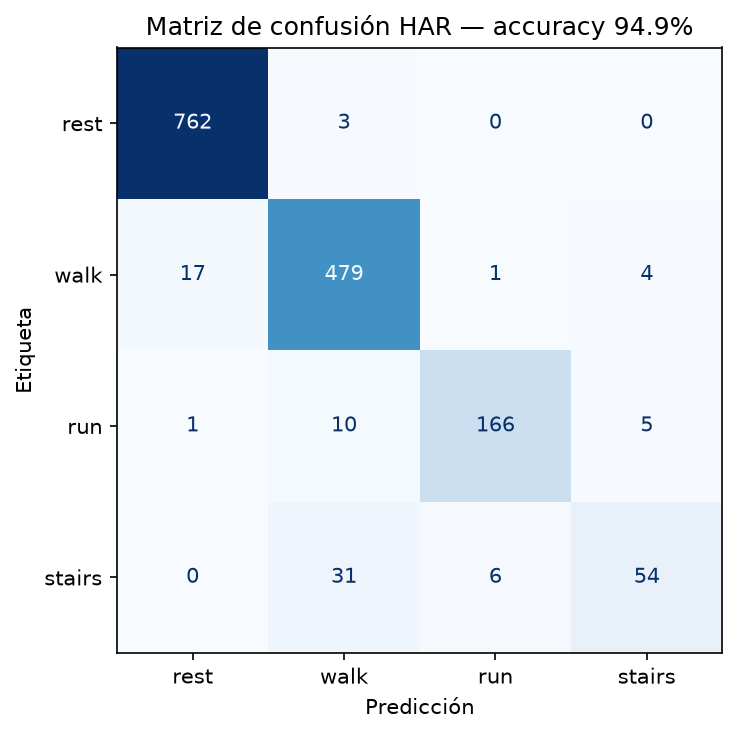
\includegraphics[width=0.93\linewidth]{har_confusion_matrix.png}
    \end{columns}
\end{frame}

% =============================================================================
\section{Especificaciones técnicas}

\begin{frame}{Diagrama de alto nivel}
    \centering
    \resizebox{0.96\textwidth}{!}{%
    \begin{tikzpicture}[
        node distance=0.55cm and 0.95cm,
        every node/.style={font=\scriptsize},
        block/.style={rectangle, rounded corners, draw=black!70, thick, fill=softgray, align=center, text width=2.8cm, minimum height=0.82cm},
        mcu/.style={rectangle, rounded corners, draw=black, thick, fill=main!18, align=center, text width=3.3cm, minimum height=1.05cm, font=\scriptsize\bfseries},
        sensor/.style={rectangle, rounded corners, draw=black!70, thick, fill=accent!14, align=center, text width=2.8cm, minimum height=0.78cm},
        bus/.style={-{Latex[length=2mm]}, thick},
        iic/.style={-{Latex[length=2mm]}, thick, main},
        spi/.style={-{Latex[length=2mm]}, thick, violet},
        adc/.style={-{Latex[length=2mm]}, thick, orange!85!black},
        ble/.style={-{Latex[length=2mm]}, thick, dashed, main}
    ]
        \node[mcu] (mcu) {XIAO ESP32-S3\\FreeRTOS + LVGL + ML};

        \node[sensor, right=1.8cm of mcu, yshift=1.85cm] (temp) {MAX30205\\temperatura};
        \node[sensor, below=0.22cm of temp] (ppg) {MAX30102\\BPM / SpO\textsubscript{2}};
        \node[sensor, below=0.22cm of ppg] (imu) {BMI160\\pasos / HAR};
        \node[sensor, below=0.22cm of imu] (touch) {Touch capacitivo\\I2C};
        \node[sensor, below=0.22cm of touch] (ecg) {AD8232\\ECG};

        \node[block, left=1.8cm of mcu, yshift=0.95cm] (lcd) {LCD táctil\\1,28''};
        \node[block, below=0.25cm of lcd] (btn) {Botones\\GPIO};

        \node[block, above=1.2cm of mcu] (pwr) {LiPo 300\,mAh\\carga/BMS XIAO};
        \node[block, below=1.25cm of mcu] (ble) {BLE NimBLE};
        \node[block, left=1.25cm of ble] (app) {App móvil\\Flutter};
        \node[block, left=1.25cm of app] (data) {Registro\\dataset};

        \draw[iic] (mcu.east) -- ++(0.45,0) |- node[near start, above]{I2C} (temp.west);
        \draw[iic] (mcu.east) -- ++(0.45,0) |- (ppg.west);
        \draw[iic] (mcu.east) -- ++(0.45,0) |- (imu.west);
        \draw[iic] (mcu.east) -- ++(0.45,0) |- (touch.west);
        \draw[adc] (mcu.east) -- ++(0.45,0) |- node[pos=0.72, below]{ADC/DMA} (ecg.west);

        \draw[spi] (mcu.west) -- ++(-0.45,0) |- (lcd.east);
        \draw[bus] (btn.east) -- ++(0.45,0) |- (mcu.west);

        \draw[bus] (pwr) -- (mcu);
        \draw[ble] (mcu) -- (ble);
        \draw[ble] (ble) -- (app);
        \draw[bus] (app) -- (data);
    \end{tikzpicture}}

    \vspace{0.15cm}
    \begin{minipage}{0.9\textwidth}
        \centering
        \scriptsize Touch capacitivo comparte el bus I2C con los sensores biométricos. App móvil y registro viajan por BLE hacia el ecosistema externo.
    \end{minipage}
\end{frame}

\begin{frame}{Uso de memoria del sistema}
    \begin{columns}[T]
        \column{0.48\textwidth}
        \centering
        \scriptsize \textbf{Flash 8\,MB} — 44\,\% ocupado\\[0.10cm]
        \begin{tikzpicture}[y=0.45cm, x=1cm]
            \fill[main]      (0,0) rectangle (2.48,1);
            \fill[accent!80] (2.48,0) rectangle (2.66,1);
            \fill[softgray]  (2.66,0) rectangle (6.00,1);
            \draw[black!25]  (0,0) rectangle (6.00,1);
            \node[font=\tiny, white] at (1.24, 0.5) {Firmware 1{,}32\,MB};
            \node[font=\tiny, black!60] at (4.33, 0.5) {Libre 6{,}5\,MB};
        \end{tikzpicture}\\[0.05cm]
        {\tiny\textcolor{accent!80}{$\blacksquare$}\,Modelo TFLite 181\,KB dentro del firmware}
        \vspace{0.35cm}

        \scriptsize \textbf{PSRAM 8\,MB} — 11\,\% asignado (890\,KB)\\[0.10cm]
        \begin{tikzpicture}[y=0.35cm, x=1cm]
            \fill[main!70]   (0,0)     rectangle (3.45,1);
            \fill[accent!80] (3.45,0)  rectangle (5.00,1);
            \fill[warn!60]   (5.00,0)  rectangle (6.00,1);
            \draw[black!25]  (0,0) rectangle (6.00,1);
            \node[font=\tiny, white] at (1.73, 0.5) {Arena HAR 512};
            \node[font=\tiny, white] at (4.22, 0.5) {LVGL 230};
            \node[font=\tiny, white] at (5.50, 0.5) {UI 150};
        \end{tikzpicture}\\[0.05cm]
        {\tiny (KB) — el 89\,\% restante queda libre para crecer}
        \column{0.52\textwidth}
        \centering
        \scriptsize \textbf{SRAM interna 512\,KB} — reparto de los 156\,KB usados\\[0.05cm]
        \begin{tikzpicture}
            \pie[
                radius=1.55, text=pin, sum=auto,
                color={main!70, accent!80, warn!70, main!30, accent!45, black!30},
                every label/.style={font=\tiny},
            ]{80/LVGL, 12/Sensores, 10/HAR, 8/UI, 6/BLE, 40/FreeRTOS}
        \end{tikzpicture}\\
        {\tiny (KB por consumidor — LVGL heap + task, HAR CNN + ring, etc.)}
        \vspace{0.05cm}
        \begin{block}{Concurrencia}
            \scriptsize La inferencia HAR queda \emph{pinned} en core 1. Sensores, BLE y UI viven en core 0 con prioridades distintas — una ventana de CNN nunca bloquea la interfaz ni las notificaciones BLE.
        \end{block}
    \end{columns}
\end{frame}

\begin{frame}{Componentes utilizados}
    \centering
    \begin{tikzpicture}[
        every node/.style={font=\scriptsize, align=center},
        card/.style={rectangle, rounded corners=3pt, draw=black!25, thick, minimum width=3.4cm, minimum height=1.55cm, inner sep=4pt},
        mcu/.style={card, fill=main!18, draw=main!60},
        bio/.style={card, fill=accent!20, draw=accent!70},
        iface/.style={card, fill=warn!15, draw=warn!60},
        pwr/.style={card, fill=softgray, draw=black!35}
    ]
        \node[mcu] (mcu) at (0,3.6) {\textbf{XIAO ESP32-S3}\\ \textit{MCU central}\\ \tiny FreeRTOS + BLE + LVGL + ML\\ \tiny (dual-core, 8\,MB PSRAM)};
        \node[bio] (max205) at (3.7,3.6) {\textbf{MAX30205}\\ \textit{Temperatura}\\ \tiny Contacto térmico con la piel};
        \node[bio] (max102) at (7.4,3.6) {\textbf{MAX30102}\\ \textit{BPM / SpO\textsubscript{2}}\\ \tiny Fotopletismografía rojo/IR};
        \node[bio] (ad8232) at (11.1,3.6) {\textbf{AD8232}\\ \textit{ECG}\\ \tiny Front-end analógico monocanal};

        \node[bio] (bmi) at (0,1.8) {\textbf{BMI160}\\ \textit{IMU}\\ \tiny Acc + gyro para pasos y HAR};
        \node[iface] (lcd) at (3.7,1.8) {\textbf{LCD táctil 1,28"}\\ \textit{Interfaz}\\ \tiny GC9A01 (SPI) + CST816S (I2C)};
        \node[pwr] (fuel) at (7.4,1.8) {\textbf{MAX17048}\\ \textit{Fuel gauge}\\ \tiny Estimación de carga y voltaje};
        \node[pwr] (lipo) at (11.1,1.8) {\textbf{LiPo 300\,mAh}\\ \textit{Energía}\\ \tiny Carga y protección en XIAO};

        \node[font=\tiny, anchor=west] at (-1.5,0.4) {\textcolor{main!70}{$\blacksquare$}\,Control};
        \node[font=\tiny, anchor=west] at (0.5,0.4) {\textcolor{accent!70}{$\blacksquare$}\,Biométricos + IMU};
        \node[font=\tiny, anchor=west] at (4.5,0.4) {\textcolor{warn!60}{$\blacksquare$}\,Interfaz de usuario};
        \node[font=\tiny, anchor=west] at (8.5,0.4) {\textcolor{black!40}{$\blacksquare$}\,Energía};
    \end{tikzpicture}
\end{frame}

\begin{frame}{Protocolos de comunicación en la PCB}
    \centering
    \begin{tikzpicture}[
        every node/.style={font=\scriptsize, align=center},
        mcu/.style={circle, draw=black, thick, fill=main!18, minimum size=1.9cm, font=\scriptsize\bfseries, align=center},
        proto/.style={rectangle, rounded corners=4pt, thick, minimum width=3.0cm, minimum height=1.20cm, inner sep=3pt, align=center},
        i2c/.style={proto, fill=main!15, draw=main!70},
        spi/.style={proto, fill=violet!15, draw=violet!70},
        adc/.style={proto, fill=orange!20, draw=orange!80!black},
        ble/.style={proto, fill=accent!20, draw=accent!70},
        gpio/.style={proto, fill=softgray, draw=black!45},
        bms/.style={proto, fill=warn!15, draw=warn!60},
        line/.style={-{Latex[length=1.7mm]}, thick}
    ]
        \node[mcu] (mcu) at (0,0) {ESP32-S3};

        \node[i2c]  (i2c)  at (-5.0, 2.0) {\textbf{I2C}\\ \tiny MAX30102 · MAX30205\\ \tiny BMI160 · MAX17048 · Touch};
        \node[spi]  (spi)  at (0, 2.4)    {\textbf{SPI}\\ \tiny LCD GC9A01 (240\,\texttimes\,240)\\ \tiny alta tasa de refresco};
        \node[adc]  (adc)  at (5.0, 2.0)  {\textbf{ADC + DMA}\\ \tiny AD8232\\ \tiny 500\,Hz sin bloquear CPU};

        \node[ble]  (ble)  at (-5.0, -2.0) {\textbf{BLE (NimBLE)}\\ \tiny Reloj $\leftrightarrow$ app Flutter\\ \tiny Telemetría + comandos};
        \node[gpio] (gpio) at (0, -2.4)   {\textbf{GPIO}\\ \tiny Botones · backlight PWM\\ \tiny wake-up deep sleep};
        \node[bms]  (bms)  at (5.0, -2.0) {\textbf{BMS integrado}\\ \tiny Carga y protección\\ \tiny (dentro del XIAO S3)};

        \draw[line, main!70]         (mcu) -- (i2c);
        \draw[line, violet!70]       (mcu) -- (spi);
        \draw[line, orange!80!black] (mcu) -- (adc);
        \draw[line, accent!70]       (mcu) -- (ble);
        \draw[line, black!45]        (mcu) -- (gpio);
        \draw[line, warn!60]         (mcu) -- (bms);
    \end{tikzpicture}
\end{frame}

\begin{frame}{Validación biométrica: resultados}
    \scriptsize
    \centering
    \renewcommand{\arraystretch}{1.25}
    \begin{tabular}{p{1.7cm}p{2.4cm}p{2.9cm}p{4.2cm}}
        \toprule
        \textbf{Métrica} & \textbf{Sensor SupaClock} & \textbf{Referencia} & \textbf{Resultado} \\
        \midrule
        BPM     & MAX30102 (PPG) & Galaxy Watch 4        & \textcolor{accent}{\textbf{$\pm$2\,\%}} de error \\
        SpO\textsubscript{2} & MAX30102 (rojo/IR) & Galaxy Watch 4 & \textcolor{accent}{\textbf{$\pm$2\,\%}} de error \\
        Temperatura & MAX30205 & Termómetro digital & 33{,}1\,\textdegree C vs 33{,}3\,\textdegree C (\textbf{0{,}2\,\textdegree C}) \\
        Pasos   & BMI160 + FFT & Conteo manual (500) & \textcolor{accent}{\textbf{$\pm$2\,\%}} de error \\
        ECG / HRV & AD8232 + Pan-Tompkins & Galaxy Watch 4 & Formas de onda similares, HRV $\pm$5\,\% \\
        \bottomrule
    \end{tabular}
    \vspace{0.35cm}
    \begin{block}{Posicionamiento}
        \scriptsize Todas las métricas caen dentro del margen aceptable para un wearable académico. La referencia comercial (Galaxy Watch 4) sirve como \emph{ground truth} dimensional, no como target clínico. La temperatura se midió en muñeca en las mismas condiciones que el sensor de contacto.
    \end{block}
\end{frame}

\begin{frame}{Contador de pasos: algoritmo FFT en el reloj}
    \centering
    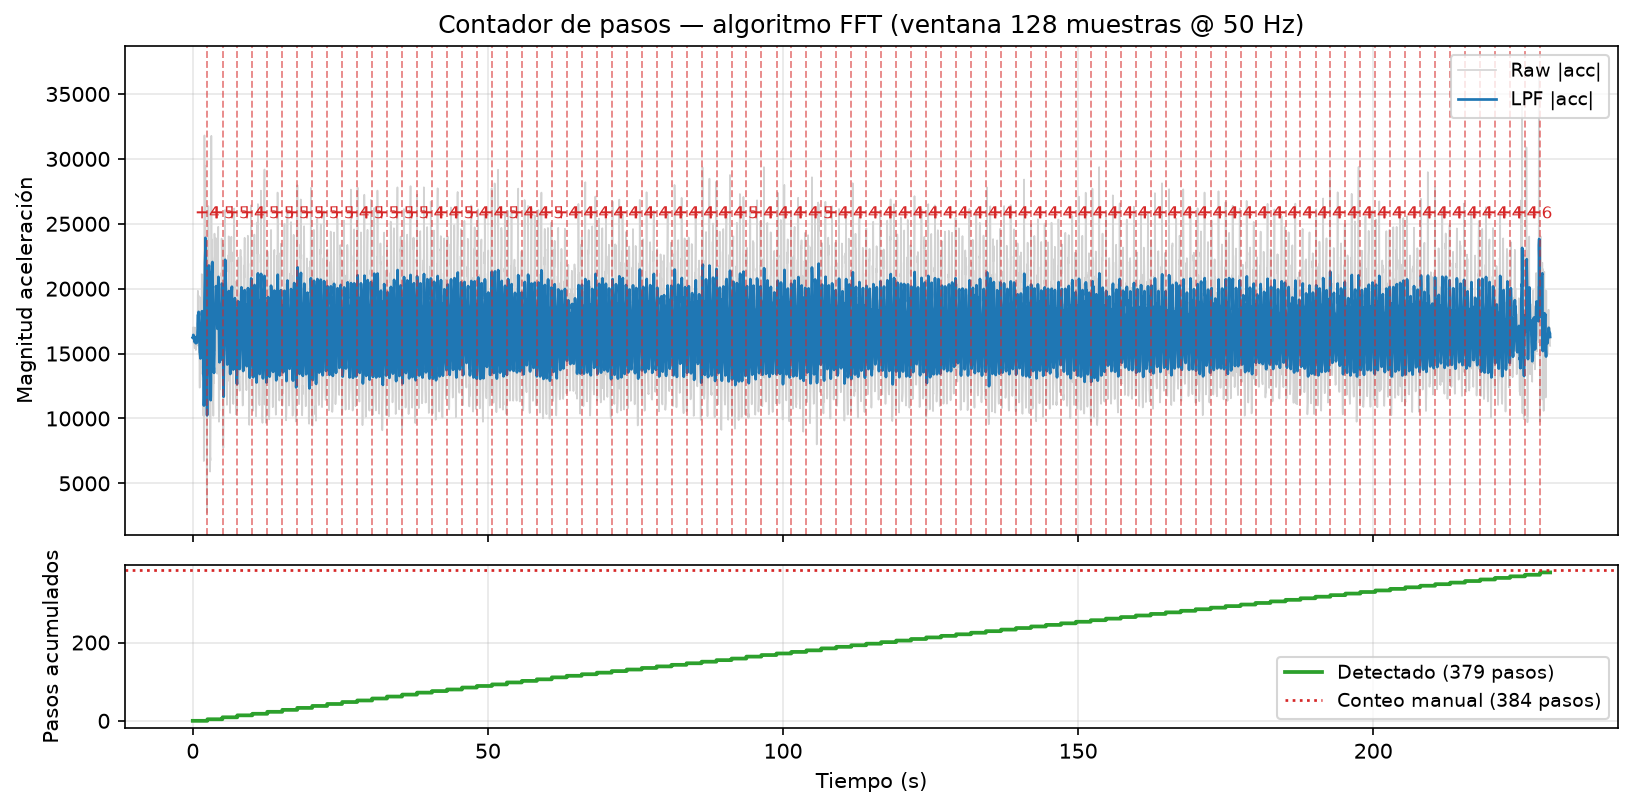
\includegraphics[width=0.90\linewidth]{grafico_pasos_s3.png}\\[0.05cm]
    \begin{minipage}{0.92\textwidth}
        \scriptsize
        Ventana FFT de 128 muestras (2,56\,s @ 50\,Hz) con Hann. Detecta la frecuencia dominante en la banda humana \textbf{1--2,5\,Hz}; pasos por ventana $= f_{\text{peak}} \times T_{\text{ventana}}$. \textbf{Resultado:} 379 detectados vs 384 manuales sobre $\sim$3,5\,min ($-$1,3\,\% de error).
    \end{minipage}
\end{frame}

\begin{frame}{ECG: adquisición y detección de picos R}
    \centering
    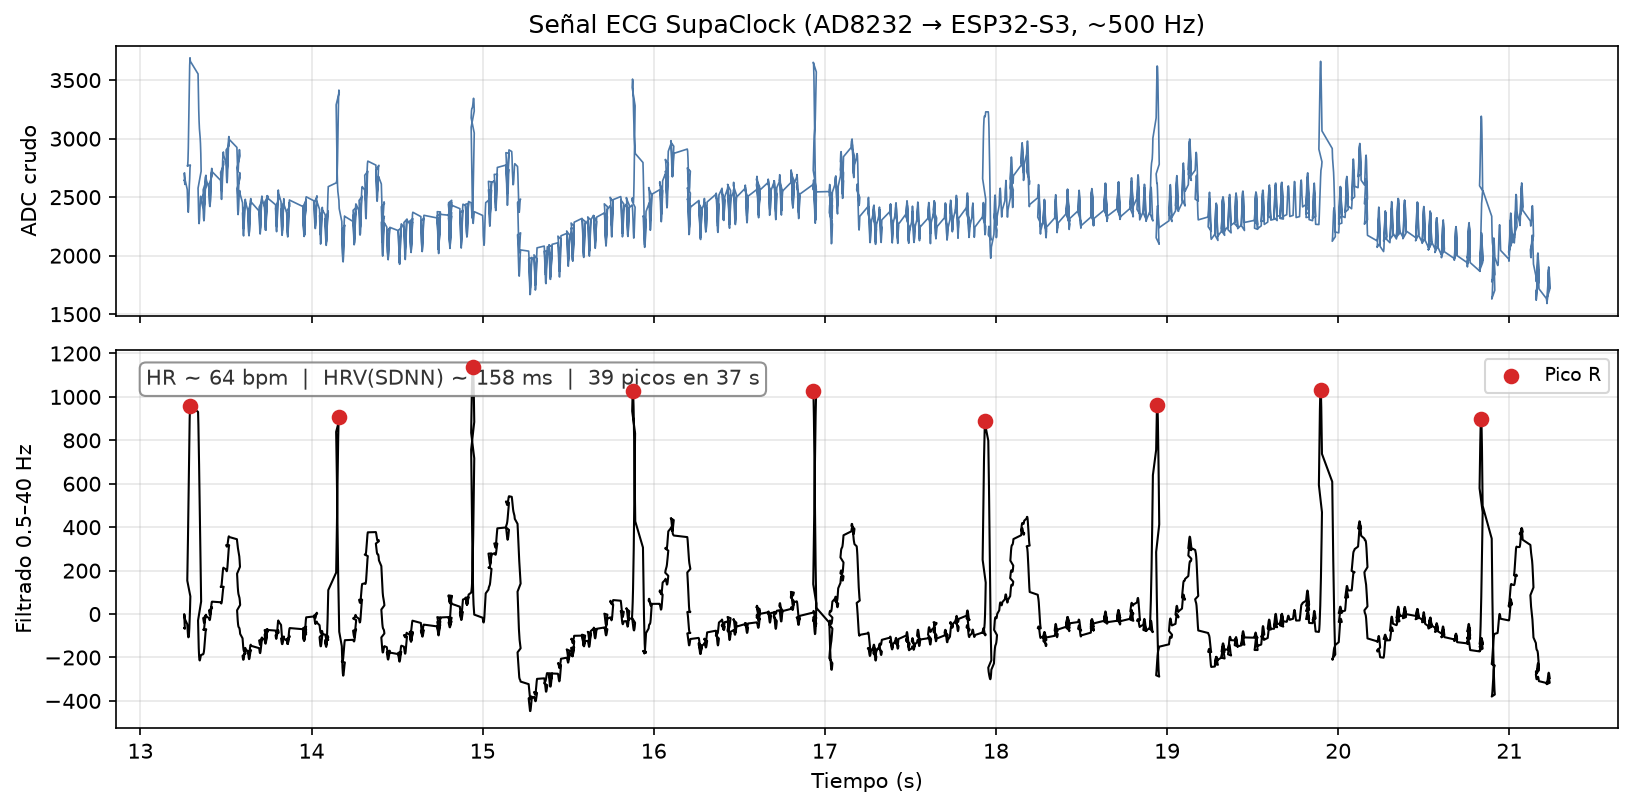
\includegraphics[width=0.90\linewidth]{grafico_ecg_supaclock.png}\\[0.05cm]
    \begin{minipage}{0.92\textwidth}
        \scriptsize
        AD8232 acondiciona la señal, ADC + DMA la muestrea a $\sim$500\,Hz sin bloquear la CPU. Pipeline Pan-Tompkins: pasabanda 0,5--40\,Hz, derivada, cuadrado e integración; picos R sobre la envolvente y refinamiento en la señal filtrada. \textbf{Sobre 37\,s:} HR $\sim$64\,bpm, HRV (SDNN) $\sim$158\,ms, 39 picos R.
    \end{minipage}
\end{frame}

\begin{frame}{Decisiones de diseño relevantes}
    \footnotesize
    \begin{columns}[T]
        \column{0.50\textwidth}
        \begin{enumerate}\itemsep0.16cm
            \item ESP32-C3 mini $\rightarrow$ XIAO ESP32-S3.
            \item PCB fabricada en China.
            \item Pantalla táctil capacitiva.
            \item Machine Learning local.
        \end{enumerate}
        \column{0.50\textwidth}
        \begin{block}{Por qué importan}
            Más cómputo, mejor integración física, menos cableado y una interfaz más natural.
        \end{block}
        \vspace{0.15cm}
        \begin{block}{Energía}
            Carga/BMS integrado y buck DC-DC reducen complejidad externa.
        \end{block}
    \end{columns}
\end{frame}

\begin{frame}{Comparación con dispositivos comerciales}
    \scriptsize
    \centering
    \renewcommand{\arraystretch}{1.20}
    \begin{tabular}{p{2.5cm}p{3.1cm}p{5.9cm}}
        \toprule
        \textbf{Dispositivo} & \textbf{Fortaleza} & \textbf{Diferencia de SupaClock} \\
        \midrule
        Apple Watch & Ecosistema maduro y sensores integrados. & Plataforma académica abierta y medible. \\
        Garmin / deportivo & Autonomía y métricas de actividad. & Enfoque biométrico compacto y validable. \\
        Oxímetro de dedo & BPM / SpO\textsubscript{2} puntual. & Integración con movimiento, app y registro. \\
        ECG portátil & Señal ECG dedicada. & ECG dentro de un wearable multipropósito. \\
        \bottomrule
    \end{tabular}
    \vspace{0.35cm}
    \begin{block}{Posicionamiento}
        \scriptsize SupaClock no busca competir como producto clínico certificado; busca demostrar integración, datos propios y validación reproducible.
    \end{block}
\end{frame}

\begin{frame}{Tabla de gastos referencial}
    \scriptsize
    \centering
    \renewcommand{\arraystretch}{1.12}
    \begin{tabular}{p{4.2cm}p{2.0cm}p{2.2cm}p{2.2cm}}
        \toprule
        \textbf{Ítem} & \textbf{Cant.} & \textbf{CLP aprox.} & \textbf{Rol} \\
        \midrule
        Seeed XIAO ESP32-S3 & 1 & 11.500 & MCU \\
        MAX17048 / fuel gauge & 1 & 3.500 & batería \\
        MAX30205 & 1 & 5.950 & temperatura \\
        MAX30102 & 1 & 1.925 & BPM/SpO\textsubscript{2} \\
        AD8232 & 1 & 7.735 & ECG \\
        BMI160 & 1 & 1.600 & IMU \\
        LCD táctil 1,28'' & 1 & 18.000 & interfaz \\
        Batería LiPo 300\,mAh & 1 & 4.000 & energía \\
        PCB fabricada & 1 & 1000 & integración \\
        Botones + misceláneos & 2+ & 100 & entrada \\
        Filamento PLA & -- & 750 & carcasa \\
        \midrule
        \textbf{Total referencial} & & \textbf{56.060} & \\
        \bottomrule
    \end{tabular}
    \vspace{0.18cm}
    \begin{minipage}{0.82\textwidth}
        \centering
        \scriptsize Valores referenciales para presentar orden de magnitud; gasto total de desarrollo: \textbf{126.980 CLP}.
    \end{minipage}
\end{frame}

\begin{frame}{Cierre}
    \begin{columns}[T]
        \column{0.55\textwidth}
        \centering
        \metric{4 clases}{$>$94\,\% val\_acc en HAR on-device}\\[0.55cm]
        \metric{$\sim$12,5\,h}{autonomía en uso mixto}\\[0.55cm]
        \metric{36\,\%}{reducción de volumen vs prototipo}\\[0.55cm]
        \metric{5 sensores}{biométricos + IMU + fuel gauge}
        \column{0.45\textwidth}
        \centering
        
\includegraphics[width=0.75\linewidth]{supaclock_logo_rayo_bn.pdf}
        \vspace{0.20cm}
        \begin{block}{Mensaje final}
            \footnotesize SupaClock demuestra que un wearable propio puede combinar biometría multi-sensor, ML on-device y ecosistema móvil sin depender de proveedor cerrado — es una plataforma abierta, medible y reproducible.
        \end{block}
    \end{columns}
\end{frame}

\end{document}
